\documentclass[a4paper]{article}

\usepackage[utf8]{inputenc}
\usepackage[T2A]{fontenc}
\usepackage[english,russian]{babel}
\usepackage{float}
\usepackage{graphicx}
\setcounter{secnumdepth}{0}

\title{Маршрутизация в компьютерной сети с применением глубокого обучения}
\author{Панчишин Иван Романович, группа М41381с}
\date{2021-06-11}

\begin{document}

\maketitle

\section{Запуск экспериментов}

Склонировать репозиторий:

\begin{verbatim}
git clone https://github.com/vpunch/routesim
\end{verbatim}

Установить пакет и зависимости в тестовое окружение:

\begin{verbatim}
python -m venv routesim-env
. routesim-env/bin/activate

cd routesim/src
python setup.py develop
pip install -r ../requirements.txt

pip install ipykernel
python -m ipykernel install --user --name=routesim-env
\end{verbatim}

Открыть нотбук:

\begin{verbatim}
cd ../notebooks
jupyter notebook
\end{verbatim}

Запустить симуляцию при помощи файла: \texttt{run\_simulation.ipynb}. 

\section{Задача 1}

Для реализации проекта был выбран язык программирования Python. Для построения
графов используется библиотека networkx, для симуляции компьютерной сети ---
simpy.

Компьютерная сеть представлена в виде графа, где в каждом узле находится
маршрутизатор.

\begin{figure}[H]
    \centering
    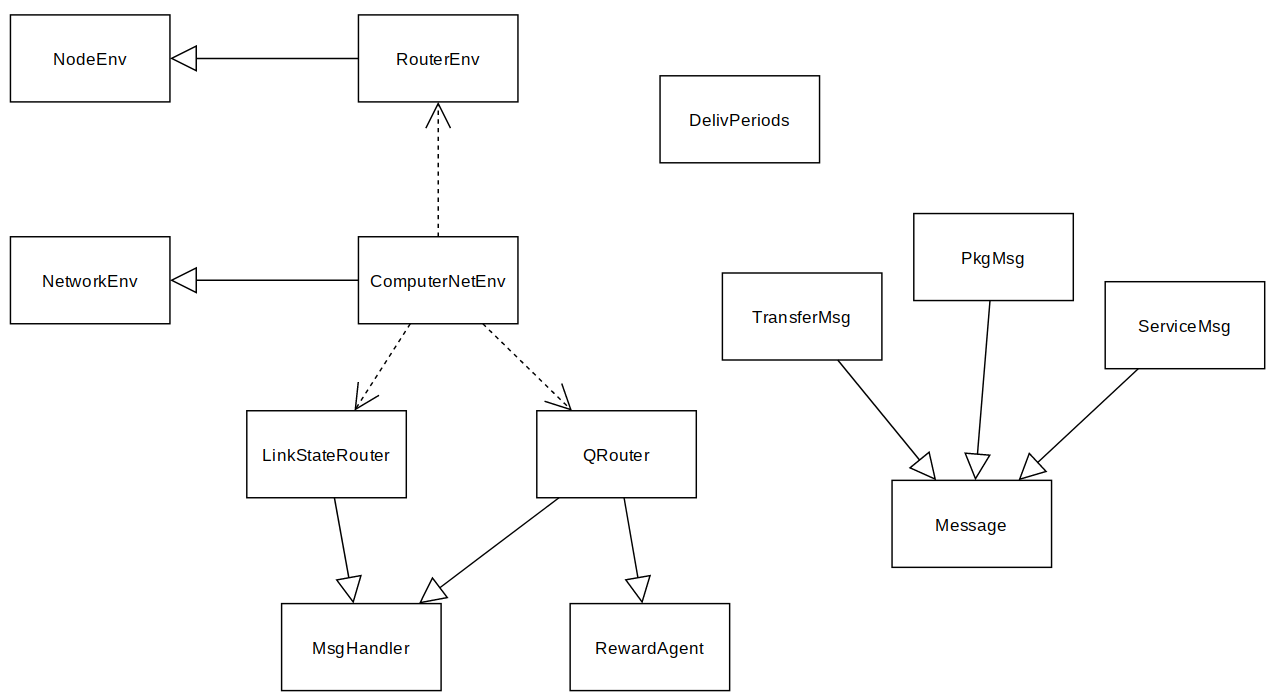
\includegraphics[width=\textwidth]{figs/classes}
    \caption{Диаграмма классов}\label{fig:cls}
\end{figure}

2 основных типа сообщений:

\begin{itemize}
    \item  Сообщение с пакетом (\texttt{PkgMsg}), перемещение которого по сети
        исследуется.

    \item Служебное сообщение (\texttt{ServiceMsg}), которым может быть анонс
        состояний в алгоритме link-state или награда в алгоритме Q.
\end{itemize}

Класс \texttt{DelivPeriods} используется для агрегации данных во время
симуляции сети.

\section{Задача 2}

Алгоритм реализован в классе \texttt{LinkStateRouter}.

\section{Задача 3}

В терминах обучения с подкреплением, маршрутизатор является агентом, сеть ---
окружением, выбор соседнего узла --- действием.

Алгоритм реализован в классе \texttt{QRouter}.

\section{Задача 4}

Эксперименты проводились в сети, которую можно представить следующим графом:

\begin{figure}[H]
    \centering
    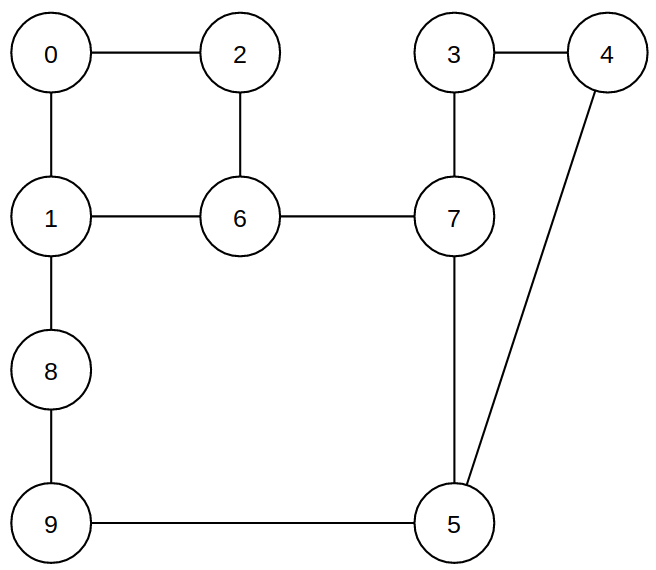
\includegraphics[width=0.4\textwidth]{figs/network}
    \caption{Структура сети}\label{fig:net}
\end{figure}

Симуляция сети выполнялась не в реальном времени, поэтому вместо секунд далее
будут указываться шаги.

Каждое ребро графа является соединением между двумя роутерами и имеет вес,
который является пропускной способностью этого соединения.

\begin{itemize}
    \item Каждое соединение имеет пропускную способность 124 байт/шаг,

    \item Каждый пакет имеет размер 1024 байт.

    \item Обработка каждого пакета роутером длится 5 шагов.
\end{itemize}

\subsection{Адаптация к изменению нагрузки на сеть}

Сценарий отправки пакетов:

\begin{itemize}
    \item 100 пакетов с задержкой 10 шагов между любыми узлами,

    \item затем 500 пакетов с задержкой 10 шагов от узлов 0, 1, 2, 6 к узлам 3,
        4, 5, 7.

    \item  затем 1500 пакетов с задержкой 5 шагов между теми же узлами,

    \item затем 500 пакетов каждые 10 шагов между теми же узлами.
\end{itemize}

Результат симуляции приведен на рисунке \ref{fig:load}.

\begin{figure}[H]
    \centering
    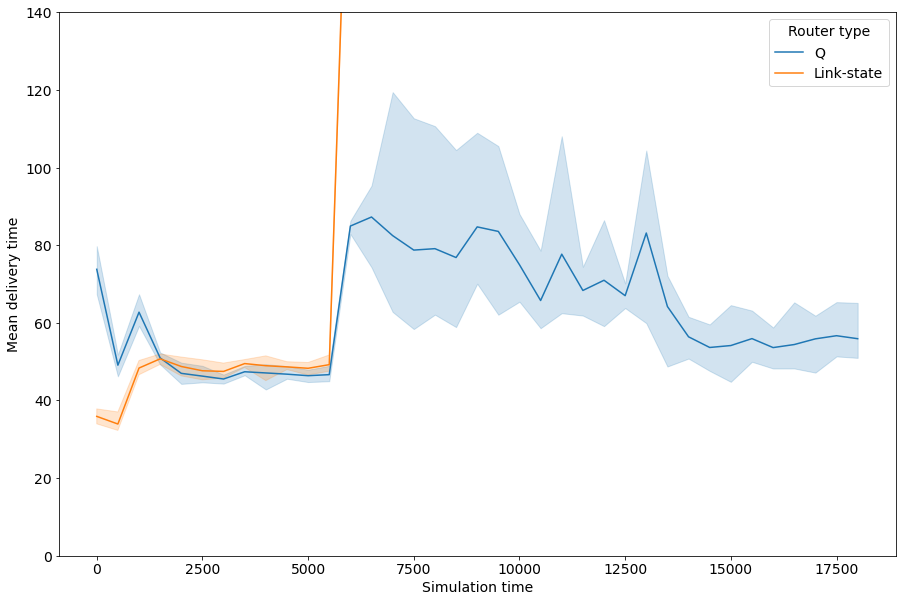
\includegraphics[width=\textwidth]{figs/load-increase}
    \caption{Изменение нагрузки}\label{fig:load}
\end{figure}

С алгоритмом link-state наблюдается быстрый рост среднего времени доставки
пакета в момент повышения нагрузки на сеть. Это связано с тем, что алгоритм
выбирает один и тот же кратчайший путь между парами узлов, основываясь только на
пропускной способности соединений, но не учитывая их
загруженность. Алгоритм Q учитывает время передачи пакета, что позволяет
изменять путь маршрутизации между парой узлов.

\subsection{Обрыв соединений}

Сценарий отправки пакетов:

\begin{itemize}
    \item 100 пакетов с задержкой 10 шагов между любыми узлами,

    \item затем 3500 пакетов с задержкой 10 шагов от узлов 0, 1, 2, 6 к узлам 3, 4,
        5, 7.
\end{itemize}

Соединения (6, 7), (0, 1), (4, 5) последовательно обрываются спустя каждые 500
пакетов, начиная со 101 пакета, затем восстанавливаются в том же порядке, с тем
же интервалом.

Результат симуляции приведен на рисунке \ref{fig:link}.

\begin{figure}[H]
    \centering
    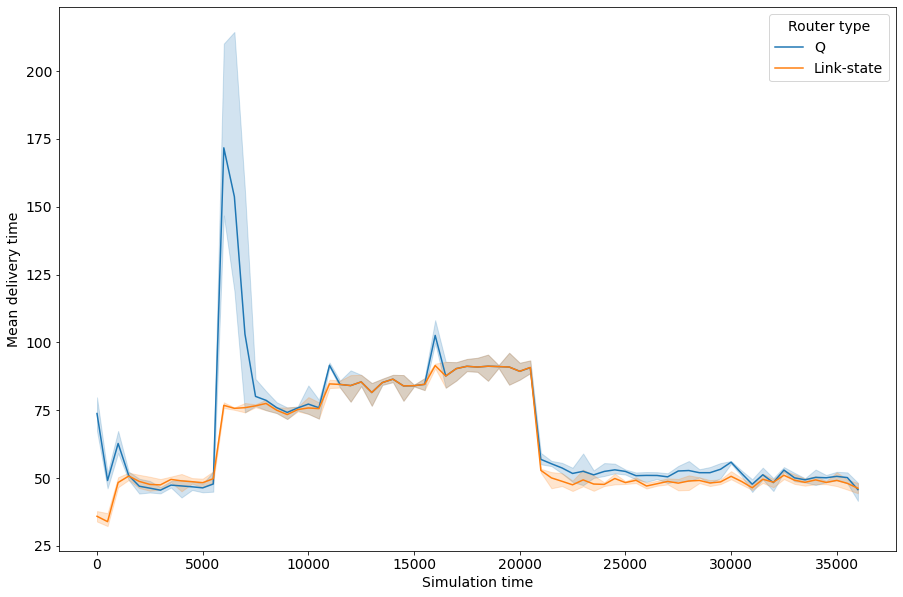
\includegraphics[width=\textwidth]{figs/link-break}
    \caption{Обрыв соединений}\label{fig:link}
\end{figure}

В алгоритме link-state маршрутизатор обновляет карту сети при каждом изменении
в своих сетевых интерфейсах. Так как служебные сообщения передаются моментально,
алгоритм мгновенно адаптируется к обрыву соединения. Алгоритму Q требуется
время для обучения, поэтому на графике наблюдается скачки среднего времени
доставки в момент обрывов и длительный возврат к оптимальной работе в момент
восстановления соединений.

\end{document}
